%% abtex2-modelo-relatorio-tecnico.tex, v-1.7.1 laurocesar
%% Copyright 2012-2013 by abnTeX2 group at http://abntex2.googlecode.com/ 
%%
%% This work may be distributed and/or modified under the
%% conditions of the LaTeX Project Public License, either version 1.3
%% of this license or (at your option) any later version.
%% The latest version of this license is in
%%   http://www.latex-project.org/lppl.txt
%% and version 1.3 or later is part of all distributions of LaTeX
%% version 2005/12/01 or later.
%%
%% This work has the LPPL maintenance status `maintained'.
%% 
%% The Current Maintainer of this work is the abnTeX2 team, led
%% by Lauro César Araujo. Further information are available on 
%% http://abntex2.googlecode.com/
%%
%% This work consists of the files abntex2-modelo-relatorio-tecnico.tex,
%% abntex2-modelo-include-comandos and abntex2-modelo-references.bib
%%

% ------------------------------------------------------------------------
% ------------------------------------------------------------------------
% abnTeX2: Modelo de Relatório Técnico/Acadêmico em conformidade com 
% ABNT NBR 10719:2011 Informação e documentação - Relatório técnico e/ou
% científico - Apresentação
% ------------------------------------------------------------------------ 
% ------------------------------------------------------------------------

% Alterado por Rodrigo Campiolo para apresentação de relatórios na disciplina
% de Redes de Computadores II do Bacharelado em Ciência da Computação da UTFPR-CM.


\documentclass[
	% -- opções da classe memoir --
	12pt,				% tamanho da fonte
	%openright,			% capítulos começam em pág ímpar (insere página vazia caso preciso)
	oneside,   	        % para impressão em verso e anverso use twoside. Oposto a oneside
	a4paper,			% tamanho do papel. 
	% -- opções da classe abntex2 --
	%chapter=TITLE,		% títulos de capítulos convertidos em letras maiúsculas
	%section=TITLE,		% títulos de seções convertidos em letras maiúsculas
	%subsection=TITLE,	% títulos de subseções convertidos em letras maiúsculas
	%subsubsection=TITLE,% títulos de subsubseções convertidos em letras maiúsculas
	% -- opções do pacote babel --
	english,			% idioma adicional para hifenização
	french,				% idioma adicional para hifenização
	spanish,			% idioma adicional para hifenização
	brazil,				% o último idioma é o principal do documento
	]{pacotes/abntex2}


% ---
% PACOTES
% ---

% ---
% Pacotes fundamentais 
% ---
\usepackage[section]{placeins}
\usepackage{algorithm}          % Escrever algoritmos
\usepackage{algpseudocode}      % Escrever algoritmos
\usepackage{cmap}				% Mapear caracteres especiais no PDF
\usepackage{lmodern}			% Usa a fonte Latin Modern
\usepackage[T1]{fontenc}		% Selecao de codigos de fonte.
\usepackage[utf8]{inputenc}		% Codificacao do documento (conversão automática dos acentos)
\usepackage{indentfirst}		% Indenta o primeiro parágrafo de cada seção.
\usepackage{color}				% Controle das cores
\usepackage{graphicx}			% Inclusão de gráficos
% ---

% ---
% Pacotes adicionais, usados no anexo do modelo de folha de identificação
% ---
\usepackage{multicol}
\usepackage{multirow}
% ---
	
% ---
% Pacotes adicionais, usados apenas no âmbito do Modelo Canônico do abnteX2
% ---
\usepackage{lipsum}				% para geração de dummy text
% ---

% ---
% Pacotes de citações
% ---
\usepackage[brazilian,hyperpageref]{backref}	 % Paginas com as citações na bibl
\usepackage[alf]{pacotes/abntex2cite}	% Citações padrão ABNT
\usepackage{comment}
% --- 
% CONFIGURAÇÕES DE PACOTES
% --- 

% ---
% Configurações do pacote backref
% Usado sem a opção hyperpageref de backref
\renewcommand{\backrefpagesname}{Citado na(s) página(s):~}
% Texto padrão antes do número das páginas
\renewcommand{\backref}{}
% Define os textos da citação
\renewcommand*{\backrefalt}[4]{
	\ifcase #1 %
		Nenhuma citação no texto.%
	\or
		Citado na página #2.%
	\else
		Citado #1 vezes nas páginas #2.%
	\fi}%
% ---

% ---
% Informações de dados para CAPA e FOLHA DE ROSTO
% ---
\titulo{Análise Empírica de Algoritmos de Subarranjo Máximo}
\autor{Allison Alfredo O Sampaio\\Mara Luci L Goulart\\Rodrigo Paula da Silva}
\local{Campo Mourão}
\data{Dezembro / 2017}
\instituicao{%
  Universidade Tecnológica Federal do Paraná -- UTFPR
  \par
  Departamento Acadêmico de Computação -- DACOM
  \par
  Bacharelado em Ciência da Computação -- BCC
}
\tipotrabalho{Relatório técnico}
% O preambulo deve conter o tipo do trabalho, o objetivo, 
% o nome da instituição e a área de concentração 
\preambulo{Relatório técnico de atividade prática solicitado pelo professor Rodrigo Campiolo na disciplina de Análise de Algoritmos do curso Bacharelado em Ciência da Computação da Universidade Tecnológica Federal do Paraná.}
% ---

% ---
% Configurações de aparência do PDF final

% alterando o aspecto da cor azul
\definecolor{blue}{RGB}{41,5,195}

% informações do PDF
\makeatletter
\hypersetup{
     	%pagebackref=true,
		pdftitle={\@title}, 
		pdfauthor={\@author},
    	pdfsubject={\imprimirpreambulo},
	    pdfcreator={LaTeX with abnTeX2},
		pdfkeywords={abnt}{latex}{abntex}{abntex2}{relatório técnico}, 
		colorlinks=true,       		% false: boxed links; true: colored links
    	linkcolor=blue,          	% color of internal links
    	citecolor=blue,        		% color of links to bibliography
    	filecolor=magenta,      		% color of file links
		urlcolor=blue,
		bookmarksdepth=4
}
\makeatother
% --- 

% --- 
% Espaçamentos entre linhas e parágrafos 
% --- 

% O tamanho do parágrafo é dado por:
\setlength{\parindent}{1.3cm}

% Controle do espaçamento entre um parágrafo e outro:
\setlength{\parskip}{0.2cm}  % tente também \onelineskip

% ---
% compila o indice
% ---
\makeindex
% ---

% Omite a numeração de capítulos
\renewcommand*\thesection{\arabic{section}}



% ----
% Início do documento
% ----
\begin{document}

% Retira espaço extra obsoleto entre as frases.
\frenchspacing 

% ----------------------------------------------------------
% ELEMENTOS PRÉ-TEXTUAIS
% ----------------------------------------------------------
% \pretextual

% ---
% Capa
% ---
%\imprimircapa
% ---

% ---
% Folha de rosto
% (o * indica que haverá a ficha bibliográfica)
% ---
\imprimirfolhaderosto
% ---


% ---
% RESUMO
% ---

% resumo na língua vernácula (obrigatório)
\begin{resumo}
A análise empírica se baseia na busca de dados relevantes e convenientes obtidos através de experências, vivência ou do pesquisar, para que assim se tenha como objetivo a chegada a novas conclusões. No relatório em questão, a análise empírica é apresentada de maneira a avaliar a performance de um algoritmo específico implementado de quatro maneiras diferentes em quatro linguagens distintas, em busca de demostrar qual deles apresenta o melhor desempenho. O algoritmo proposto para a análise dispõe-se a encontrar uma sublista contígua de maior soma a partir de uma lista de números inteiros, as linguagens de programação usadas para a implementação foram C, Python, Java e Ruby. A entrada apresenta um conjunto de valores aleatórios, mistos entre positivos e negativos, as mesmas foram utilizadas em todos os algoritmos. Os resultados obtidos são apresentados ao decorrer do relatório, a análise compara o tempo pelo tamanho das entradas e se constitui de duas formas, a implementação de quatro algoritmos em uma linguagem específica de programação e a implementação em cada linguagem de programação para um algoritmo específico.

 \vspace{\onelineskip}
    
 \noindent
 \textbf{Palavras-chave}: analise empirica. analise de algoritmos.  
\end{resumo}
% ---

% ---
% inserir lista de ilustrações
% ---
%\pdfbookmark[0]{\listfigurename}{lof}
%\listoffigures*
%\cleardoublepage
% ---

% ---
% inserir lista de tabelas
% ---
%\pdfbookmark[0]{\listtablename}{lot}
%\listoftables*
%\cleardoublepage
% ---

% ---
% inserir lista de abreviaturas e siglas
% ---
%\begin{siglas}
%  \item[IP] Internet Protocol
%  \item[TCP] Transmission Control Protocol
%  \item[UDP] User Datagram Protocol
%\end{siglas}
% ---

% ---
% inserir o sumario
% ---
\pdfbookmark[0]{\contentsname}{toc}
\tableofcontents*
\cleardoublepage
% ---

% ----------------------------------------------------------
% ELEMENTOS TEXTUAIS
% ----------------------------------------------------------
\textual

\makeatletter
\renewcommand{\chapter}{\@gobbletwo}
\makeatother

\section{Introdução}
\label{sec:introducao}

% ÍNICIO DE INTRODUÇÃO

A análise empírica visa auxiliar na avaliação de eficiência de um algoritmo, uma das medidas de eficiência é o tempo de execução. O tempo de execução geralmente varia de acordo com o tamanho das entradas \cite{silva:12}.
A análise foi feita sobre o problema do subvetor máximo, que consiste em encontrar a maior soma em um vetor com números negativos e positivos \cite{goodrich:02}.
Uma das soluções implementadas  é a divisão e conqusita na qual a instância dada do problema é dividida em duas ou mais instâncias menores, cada instância menor é resolvida usando o próprio algoritmo  as soluções das instâncias menores são combinadas e então retornam com a solução da instância original \cite{feofiloff:03}.
Outra solução interessante é a programação dinâmica, aplicada quando o problema possui estrutura recursiva \cite{feofiloff:03}.
As soluções apresentadas foram implementadas nas linguagens de programação C, Python, Java e Ruby.
O relatório está organizado da seguinte forma: na seção 2 é apresentado o objetivo, ou seja, medir a eficiência das implementações de acordo com o tempo de execução; na seção 3 é apresentada a fundamentação teórica dos conceitos presentes no trabalho; na seção 4 é descrito os materiais que foram utilizados; na seção 5 os  resultados que foram obtidos após executar os quatro algoritmos em suas respectivas linguagens; na seção 6 a disussão dos resultados que foram conquistados; na seção 7 a conclusão ; na seção 8 as referências utilizadas e por fim nos apêndices se encontram os resultados detalhados de cada algoritmo em cada uma das linguagens.


\section{Objetivos}
\label{sec:objetivos}
O objetivo deste trabalho é realizar a análise empírica de quatro algorítmos que utilizam os conceitos de: laços de repetição por força bruta (enumeration e better enumeration), divisão e conquista, e programação dinâmica. As entradas possuem os seguintes tamanhos, calculados a partir da potência de 2: $2^7 (128)$, $2^8(256)$, $2^9(512)$, $2^{10}(1024)$, $2^{11}(2048)$, $2^{12}(4096)$. Após executar 5 entradas diferentes para cada tamanho calculou-se a média de tempo em milisegundos.

\section{Fundamentação}
\label{sec:fundamentacao}
\subsection{Análise Empírica}
A análise empírica visa mensurar a eficiência de um algoritmo, geralmente por meio do tempo de execução,
considerando tempo de relógio como tempo de CPU. Essa medição se dá pela contagem de vezes que cada instrução
no código é executada \cite{heineman:16}. Por meio dessa análise é possível detectar os pontos de melhoria necessário no algoritimo
testado.
Além da eficiência das intruções do código, ressalta-se que o hardware utilizado influencia no tempo de execução
bem como no uso da memória \cite{heineman:16}.
Os principais objetivos da análise empírica são: avaliar a corretude dos algoritmos, comparar a eficiência de diferentes algoritmos, comparar implementações alternativas do mesmo algoritmo, identificar a complexidade do algoritmo \cite{bentley:84}. 

\subsection{Subvetor Máximo}
No problema do subvetor máximo, temos um vetor com números inteiros positivos e negativos, e esperamos como saída a maior soma em um intervalo \cite{heineman:16}.

\begin{verbatim}
   s j,k = a j + a j+1 + · · · + a k 
\end{verbatim}

Dentre os tipos de implementação do subvetor máximo estão o \textit{enumeration}, \textit{better enumeration}, \textit{divisão e conquista}, e \textit{programação dinâmica}, conforme descritos a seguir:

 \begin{itemize}
   \item Enumeration: Loop para cada par de indices i,j calculando a soma de a[k] tendo k=i até k=j e guardando a melhor soma encontrada até agora.
   
   \item Better Enumeration: Observe que no algoritmo anterior, a mesma soma é calculada muitas vezes. Em particular, observe que é calculado a soma de a[k] tendo k=i até k=j, isso pode ser calculado como a soma de a[k] tendo k=i até k=(j-1), sendo uma nova versão do primeiro algoritmo que aproveite esta observação.
   
   \item Divisão e Conquista: Se dividimos a entrada em duas metades, sabemos que a maior soma estará contida inteiramente na primeira parte, contida inteiramente na segunda parte ou começando na primeira parte e terminando na segunda. Os dois primeiros casos podem ser encontrados recursivamente. O último caso pode ser encontrado em tempo linear.
   
   \item Programação Dinâmica: O subarray máximo pode ou não usar o último elemento da entrada.
   
 \end{itemize}

\subsection{Linguagens de Programação}
A escolha das linguagens de programação utilizadas na implementação dos algoritmos se baseia nos conhecimentos prévios dos autores do relatório em questão. São elas:
 \begin{itemize}
   \item C: Linguagem de programação compilada de propósito geral, estruturada, imperativa, procedural, padronizada pela ISO, criada em 1972, por Dennis Ritchie, no AT&T Bell Labs, para desenvolver o sistema operacional Unix \cite{c:17}.
   \item Python: Linguagem de programação de alto nível, interpretada, de script, imperativa, orientada a objetos, funcional, de tipagem dinâmica e forte. Foi lançada por Guido van Rossum em 1991. Atualmente possui um modelo de desenvolvimento comunitário, aberto e gerenciado pela organização sem fins lucrativos Python Software Foundation \cite{python:17}.
   \item Java: Linguagem de programação interpretada orientada a objetos desenvolvida na década de 90 por uma equipe de programadores chefiada por James Gosling. Diferente das linguagens de programação convencionais, que são compiladas para código nativo, a linguagem Java é compilada para um bytecode que é interpretado por uma máquina virtual \cite{java:17}.
   \item Ruby: Linguagem de programação interpretada multiparadigma, de tipagem dinâmica e forte, com gerenciamento de memória automático, originalmente planejada e desenvolvida no Japão em 1995, por Yukihiro "Matz" Matsumoto, para ser usada como linguagem de script \cite{ruby:17}.
 \end{itemize}

\section{Materiais}
\label{sec:materiais}
O material necessário para a execução dos algoritmos e coleta de dados foi um notebook com as seguintes especificações:
 \begin{itemize}
   \item Sistema operacional: Ubuntu 16.04.3 LTS (Xenial)
   \item Processador: Intel(R) Core(TM) i3-4010U CPU @ 1.70GHz (4 CPUs)
   \item Memória: 4 GB
   \item Compiladores: GCC 5.4.0 / Java 1.8 / Python 3.5 / Ruby 2.3.1p112
 \end{itemize}


\section{Procedimentos e Resultados}
\label{sec:procedimentos}

O  procedimento utilizado para realizar a análise empírica, foi a implementação dos algoritmos
nas linguagens propostas junto com uma função de medição de tempo de execução.
Após executar cinco vezes cada algoritmo em suas respectivas linguagens para seis tamanhos
diferentes determinados a partir da potência de  $2^{n}$, coletamos os dados e geramos os gráficos
presentes nesta seção.

\newpage
\subsection{Análise Matemática}
A seguir são apresentados os pseudocódigos dos algoritmos utilizados na análise.

\subsubsection{Algoritmo enumeration}
\begin{algorithm}
\caption{Enumeration}
\label{algo:preencheprimeiroarranjo}
\begin{algorithmic}[1]
    \Function{enumeratio}{$v$}
        \State  $soma \gets 0$
        \State $max \gets v[1]$
        \For{i in 1..n}
            \For{j in i..n}
                \For{k in i..j}
                    \State $soma \gets soma+v[k]$
                \EndFor
                \If{$soma > max$}
                    \State $max \gets soma$
                    \State $start, end \gets i, j$
                \EndIf
            \EndFor
        \EndFor
        \State \Return $(max, start, end)$
    \EndFunction
\end{algorithmic}
\end{algorithm}

\paragraph{Análise assintótica} Cada laço \textit{for} executa em tempo $O(n)$, portanto o tempo de execução do algoritmo no pior caso é $O(n^3)$.

\subsubsection{Algoritmo better enumeration}
\begin{algorithm}
\caption{Better Enumeration}
\label{algo:preencheprimeiroarranjo}
\begin{algorithmic}[1]
    \Function{better-enumeration}{$v$}
        \State  $soma \gets 0$
        \State $max \gets v[1]$
        \For{i in 1..n}
            \For{j in i..n}
                \State $soma \gets soma+v[j]$
                \If{$soma > max$}
                    \State $max \gets soma$
                    \State $start, end \gets i, j$
                \EndIf
            \EndFor
        \EndFor
        \State \Return $(max, start, end)$
    \EndFunction
\end{algorithmic}
\end{algorithm}

\paragraph{Análise assintótica} Como são dois laços \textit{for} aninhados e cada um executa em tempo $O(n)$, o tempo de execução do algoritmo no pior caso é $O(n^2)$.

\subsubsection{Algoritmo divisão e conquista}
\begin{algorithm}
\caption{divisão e conquista}
\label{algo:preencheprimeiroarranjo}
\begin{algorithmic}[1]
    \Function{max-cross}{$A, e, m, d$}
        \State $l\_sum \gets -\infty$
        \State  $sum \gets 0$
        \For{$\forall i \in m..e$}
            \State $sum \gets sum+A[i]$
            \If{$sum>l\_sum$}
                \State $l\_sum \gets sum$
                \State $max\_l \gets i$
            \EndIf
        \EndFor
        \State $r\_sum \gets +\infty$
        \State $sum \gets 0$
        \For{$\forall j \in (m+1)..d$}
            \State $sum \gets sum+A[j]$
            \If{$sum>r\_sum$}
                \State $r\_sum \gets sum$
                \State $max\_r \gets j$
            \EndIf
        \EndFor
        \State \Return $(max\_l, max\_r, l\_sum+r\_sum)$
    \EndFunction
    \State
    \Function{max-subarray}{$A,e,d$}
        \If{e = d}
            \State \Return $(e,d,A[e])$
        \EndIf
        \State $m \gets \lfloor(e+d)/2\rfloor$
        \State $(l\_esq, l\_dir, l\_sum) \gets$ MAX-SUBARRAY$(A,e,m)$
        \State $(r\_esq, r\_dir, r\_sum) \gets$ MAX-SUBARRAY$(A,m+1,d)$
        \State $(c\_esq, c\_dir, c\_sum) \gets$ MAX-CROSS$(A,e,m,d)$
        \If{$(l\_sum \geq r\_sum) \land (l\_sum \geq c\_sum)$}
            \State \Return $(l\_esq, l\_dir, l\_sum)$
        \ElsIf{$(r\_sum \geq l\_sum) \land (r\_sum \geq c\_sum)$}
            \State \Return $(r\_esq, r\_dir, r\_sum)$
        \Else
            \State \Return $(c\_esq, c\_dir, c\_sum)$
        \EndIf
    \EndFunction
\end{algorithmic}
\end{algorithm}

\paragraph{Análise assintótica} Cada chamada de MAX-SUBARRAY executa em tempo $T(n) = T(n/2)$, e o procedimento MAX-CROSS em tempo $\theta(n)$, portanto a recorrência do algoritmo é dada por: $T(n) = 2T(n/2) + \theta(n)$. Pelo método mestre,  $T(n) = \theta(n\log{n})$ para o pior caso.

\subsubsection{Programação dinâmica}

\begin{algorithm}
\caption{programação dinâmica (Kadane's algorithm)}
\label{algo:preencheprimeiroarranjo}
\begin{algorithmic}[1]
    \Function{max-subarray}{$v$}
        \State $current \gets maximum \gets v[1]$
        \For{$\forall x \in v$}
            \State $current \gets max(x, current + x)$
            \State $maximum \gets max(maximum, current)$
        \EndFor
        \State \Return maximum
    \EndFunction
\end{algorithmic}
\end{algorithm}

\paragraph{Análise assintótica} Tempo de execução no pior caso: $O(n)$.

\FloatBarrier
\subsection{Resultados Python}


A Tabela \ref{tab:python} apresenta a média de tempo dos resultados da execução de cada algoritmo em Python:

\begin{table}[!htb]
\centering
\caption{Tempo em milisegundos utilizando cada algoritmo em Python}
\label{tab:python}
\footnotesize   %%diminuir tamanho do fonte (-2)
%\small          %%diminuir tamanho de fonte (-1)
\begin{tabular}{l|llllll}
\toprule
\textbf{} & $2^7$ & $2^8$ & $2^9$ & $2^{10}$ & $2^{11}$ & $2^{12}$\\
\midrule
\textbf{Enumeration} & 41,9128 & 317,2804 & 2720,5762 & 22657,0328 & 184467,2862 & 1492802,713\\
\textbf{Better Enumeration} & 4,1868038 & 17,1467958 & 68,5272922 & 271,4727162 & 1088,7628242 & 4320,3160314\\
\textbf{Divide and Conquer} & 0,7718672 & 1,6408722 & 3,5756074 & 7,6058672 & 16,4137414 & 34,952661\\
\textbf{Dynamic} & 0,1008058 & 0,1776342 & 0,3386812 & 0,7952252 & 1,2868458 & 2,595719\\
\bottomrule
\end{tabular}
\end{table}

\subsection{Resultados C}


A Tabela \ref{tab:c} apresenta a média de tempo dos resultados da execução de cada algoritmo em C:

\begin{table}[!htb]
\centering
\caption{Tempo em milisegundos utilizando cada algoritmo em C}
\label{tab:c}
\footnotesize   %%diminuir tamanho do fonte (-2)
%\small          %%diminuir tamanho de fonte (-1)
\begin{tabular}{l|llllll}
\toprule
\textbf{} & $2^7$ & $2^8$ & $2^9$ & $2^{10}$ & $2^{11}$ & $2^{12}$\\
\midrule
\textbf{Enumeration} & 2,8864 & 16,5286 & 119,8916 & 939,4412 & 7479,771 & 55494,3894\\
\textbf{Better Enumeration} & 0,0426 & 0,1608 & 0,63 & 2,4924 & 9,945 & 39,711\\
\textbf{Divide and Conquer} &0,0198 & 0,038 & 0,0728 & 0,1486 & 0,3014 & 0,6196\\
\textbf{Dynamic} & 0,007 & 0,0126 & 0,0234 & 0,0408 & 0,0836 & 0,2528\\
\bottomrule
\end{tabular}
\end{table}


\subsection{Resultados Java}

A Tabela \ref{tab:java} apresenta a média de tempo dos resultados da execução de cada algoritmo em Java:

\begin{table}[!htb]
\centering
\caption{Tempo em milisegundos utilizando cada algoritmo em Java}
\label{tab:java}
\footnotesize   %%diminuir tamanho do fonte (-2)
%\small          %%diminuir tamanho de fonte (-1)
\begin{tabular}{l|llllll}
\toprule
\textbf{} & $2^7$ & $2^8$ & $2^9$ & $2^{10}$ & $2^{11}$ & $2^{12}$\\
\midrule
\textbf{Enumeration} & 8,4 & 16,6 & 49 & 223,6 & 1730,8 & 13050,6\\
\textbf{Better Enumeration} & 3,4 & 4,6 & 9,2 & 16,4 & 24,2 & 60,6\\
\textbf{Divide and Conquer} & 3,8 & 4,2 & 6,2 & 7,4 & 7,6 & 9\\
\textbf{Dynamic} & 3,4 & 3,8 & 4,6 & 5,2 & 5 &5,4\\
\bottomrule
\end{tabular}
\end{table}

\subsection{Resultados Ruby}

A Tabela \ref{tab:ruby} apresenta a média de tempo dos resultados da execução de cada algoritmo em Ruby:

\begin{table}[!htb]
\centering
\caption{Tempo em milisegundos utilizando cada algoritmo em Ruby}
\label{tab:ruby}
\footnotesize   %%diminuir tamanho do fonte (-2)
%\small          %%diminuir tamanho de fonte (-1)
\begin{tabular}{l|llllll}
\toprule
\textbf{} & $2^7$ & $2^8$ & $2^9$ & $2^{10}$ & $2^{11}$ & $2^{12}$\\
\midrule
\textbf{Enumeration} & 37,2079984 & 295,3568084 & 2053,3077692 & 17024,4681768 & 126279,8878782 & 1003486,1794356\\
\textbf{Better Enumeration} & 1,0114974 & 4,0858984 & 15,8537784 & 62,529755 & 262,2592524 & 985,6924684\\
\textbf{Divide and Conquer} & 0,3232428 & 0,764659 & 1,5209966 & 3,0886588 & 6,1329074 & 12,4267286\\
\textbf{Dynamic} & 0,0236498 & 0,0464976 & 0,0893338 & 0,1851136 & 0,3241004 & 0,7343924\\
\bottomrule
\end{tabular}
\end{table}

\newpage
\section{Discussão dos Resultados}
\label{sec:discussao}

O  procedimento utilizado para realizar a análise empírica, foi a implementação dos algoritmos
nas linguagens propostas junto com uma função de medição de tempo de execução.
Após executar cinco vezes cada algoritmo em suas respectivas linguagens para seis tamanhos
diferentes determinados a partir da potência de  $2^{n}$, coletamos os dados e geramos os gráficos
presentes nesta seção.

Os gráficos a seguir apresentam uma comparação entre as linguagens utilizadas:

\begin{center}
    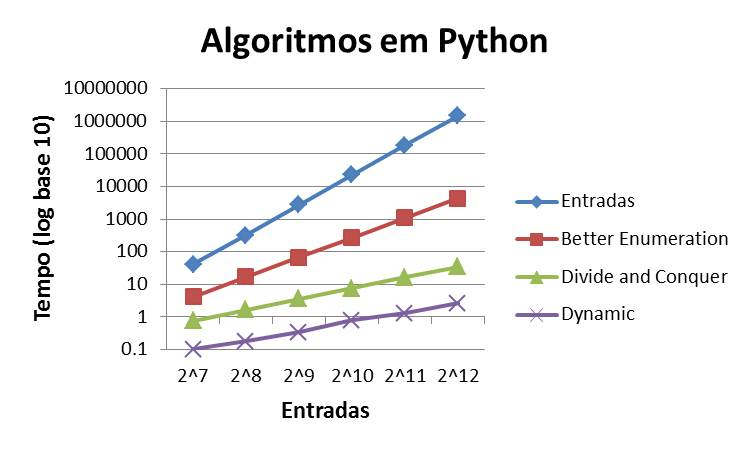
\includegraphics[scale=0.9]{figuras/python.jpg}\\
    \caption{Figura 1: Média do tempo de execução em Python}
\end{center}

\begin{center}
    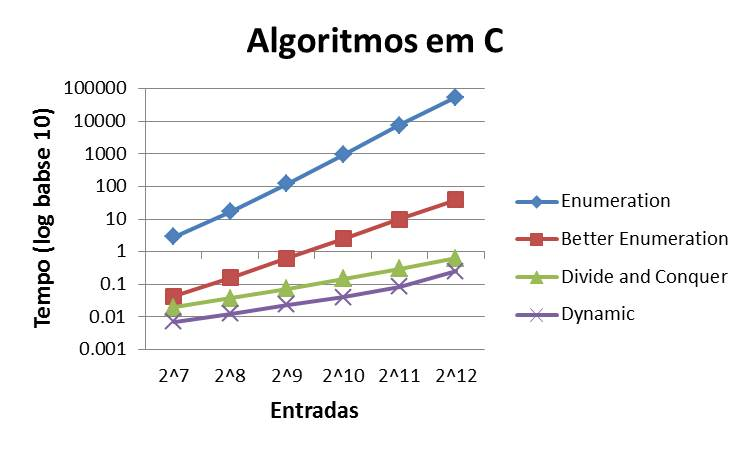
\includegraphics[scale=0.9]{figuras/c.jpg}\\
    \caption{Figura 2: Média do tempo de execução em C}
\end{center}

\begin{center}
    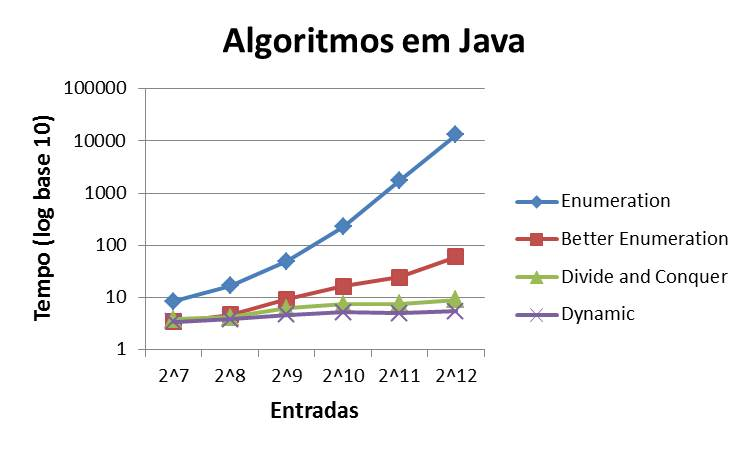
\includegraphics[scale=0.9]{figuras/java.jpg}\\
    \caption{Figura 3: Média do tempo de execução em Java}
\end{center}

\begin{center}
    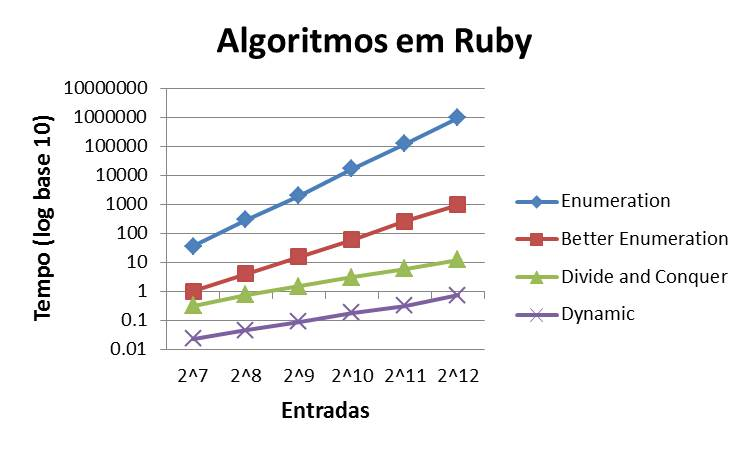
\includegraphics[scale=0.9]{figuras/ruby.jpg}\\
    \caption{Figura 4:Média do tempo de execução em Ruby}
\end{center}


% tabelas algoritmos

As tabelas \ref{tab:enumeration},\ref{tab:betterenumeration},\ref{tab:divideandconquer} e \ref{tab:dynamic} apresentam a comparação entre as linguagens na implementação de cada algoritmo.

\begin{table}[!htb]
\centering
\caption{Enumeration}
\label{tab:enumeration}
\footnotesize   %%diminuir tamanho do fonte (-2)
%\small          %%diminuir tamanho de fonte (-1)
\begin{tabular}{l|llllll}
\toprule
& \textbf{$2^7$} & \textbf{$2^8$} & \textbf{$2^9$} & \textbf{$2^{10}$} & \textbf{$2^{11}$} & \textbf{$2^{12}$}\\ 
\midrule
\textbf{Python} &  41.9128 & 317.2804 & 2720.5762 & 22657.03218 & 184467.2862 & 1492802.713 \\
\textbf{C} & 2.8864 & 16.5286 & 119.8916 & 939.4412 & 7479.771 & 55494.3894 \\
\textbf{Java} & 8.4 & 16.6 & 49 & 223.6 & 1730.8 & 13050.6 \\
\textbf{Ruby} &  37.2079984 & 295.3568084 & 2053.307769 & 17024.46818 & 126279.8879 & 1003486.179\\
 \bottomrule
\end{tabular}
\end{table}


\begin{table}[!htb]
\centering
\caption{Better Enumeration}
\label{tab:betterenumeration}
\footnotesize   %%diminuir tamanho do fonte (-2)
%\small          %%diminuir tamanho de fonte (-1)
\begin{tabular}{l|llllll}
\toprule
& \textbf{$2^7$} & \textbf{$2^8$} & \textbf{$2^9$} & \textbf{$2^{10}$} & \textbf{$2^{11}$} & \textbf{$2^{12}$}\\ 
\midrule
\textbf{Python} & 4.1868038 & 17.1467958 & 68.527922 & 271.4727162 & 1088.762824 & 4320.316031 \\
\textbf{C} &  0.0426 & 0.1608 & 0.63 & 2.4924 & 9.945 & 39.711\\
\textbf{Java} & 3.4 & 4.6 & 9.2 & 16.4 & 24.2 & 60.6 \\
\textbf{Ruby} & 1.0114974 & 4.0858984 & 15.8537784 & 62.529755 & 262.2592524 & 985.6924684 \\
 \bottomrule
\end{tabular}
\end{table}

\begin{table}[!htb]
\centering
\caption{Divisão e Conquista}
\label{tab:divideandconquer}
\footnotesize   %%diminuir tamanho do fonte (-2)
%\small          %%diminuir tamanho de fonte (-1)
\begin{tabular}{l|llllll}
\toprule
& \textbf{$2^7$} & \textbf{$2^8$} & \textbf{$2^9$} & \textbf{$2^{10}$} & \textbf{$2^{11}$} & \textbf{$2^{12}$}\\ 
\midrule
\textbf{Python} &  0.7718672 & 1.6408722 & 3.5756074 & 7.6058672 & 16.4137414 & 34.952661\\
\textbf{C} & 0.0198 & 0.038 & 0.0728 & 0.1486 & 0.3014 & 0.6196 \\
\textbf{Java} & 3.8 & 4.2 & 6.2 & 7.4 & 7.6 & 9 \\
\textbf{Ruby} &  0.3232428 & 0.764659 & 1.5209966 & 3.0886588 & 6.1329074 & 12.4267286\\
 \bottomrule
\end{tabular}
\end{table}

\begin{table}[!htb]
\centering
\caption{Dinâmico}
\label{tab:dynamic}
\footnotesize   %%diminuir tamanho do fonte (-2)
%\small          %%diminuir tamanho de fonte (-1)
\begin{tabular}{l|llllll}
\toprule
& \textbf{$2^7$} & \textbf{$2^8$} & \textbf{$2^9$} & \textbf{$2^{10}$} & \textbf{$2^{11}$} & \textbf{$2^{12}$}\\ 
\midrule
\textbf{Python} &  0.1008058 & 0.1776342 & 0.3386812 & 0.7952252 & 1.2868458 & 2.595719\\
\textbf{C} & 0.007 & 0.0126 & 0.0234 & 0.0408 & 0.0836 & 0.2518 \\
\textbf{Java} & 3.4 & 3.8 & 4.6 & 5.2 & 5.0  & 5.4 \\
\textbf{Ruby} &  0.0236498 & 0.0464976 & 0.0893338 & 0.181136 & 0.3241004 & 0.7343924\\
 \bottomrule
\end{tabular}
\end{table}

%%%%%%%%%%%%%%%%%%%%%

\begin{center}
    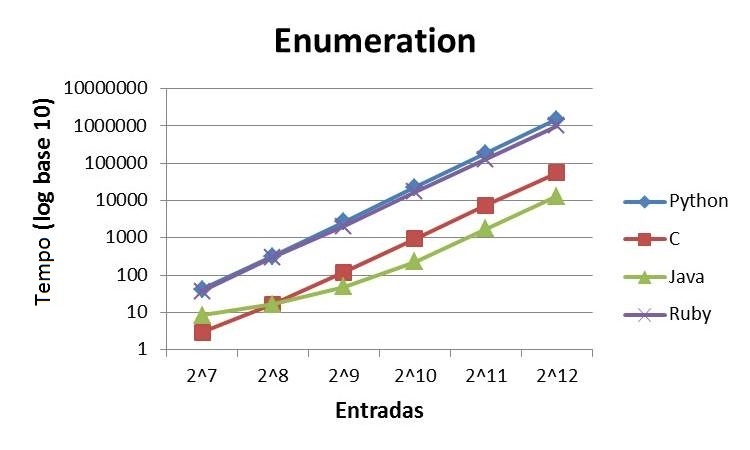
\includegraphics[scale=0.9]{figuras/enumeration.jpg} \\
    \caption{Figura 5: Tempo de execução Enumeration}
\end{center}

\begin{center}
    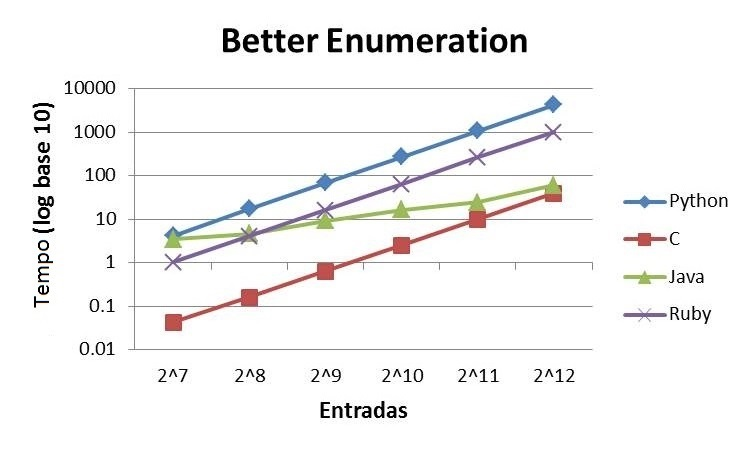
\includegraphics[scale=0.9]{figuras/better-enumeration.jpg} \\
    \caption{Figura 6: Tempo de execução Better Enumeration}
\end{center}

\begin{center} 
    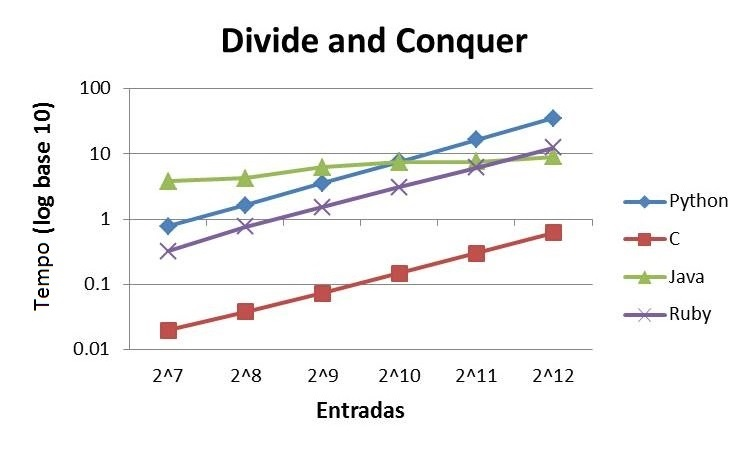
\includegraphics[scale=0.9]{figuras/divide-conquer.jpg} \\
    \caption{Figura 7: Tempo de execução Divide and Conquer}
\end{center}

\begin{center}
    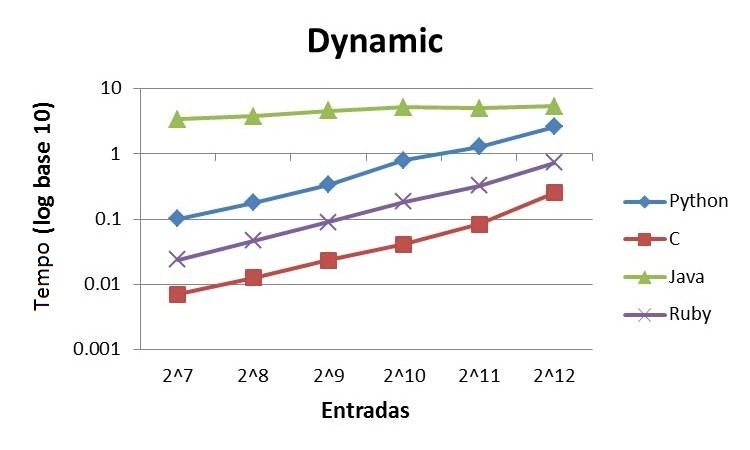
\includegraphics[scale=0.9]{figuras/dynamic.jpg} \\
    \caption{Figura 8: Tempo de execução Dynamic}
\end{center}


O gráfico a seguir mostra a relação entre a complexidade de cada algoritmo e a linguagem na qual cada um foi implementado e seus respectivos tempos de execução, utilizando o a média dos tempos de execução com o tamanho do vetor $2^{12}$.

\begin{center}
    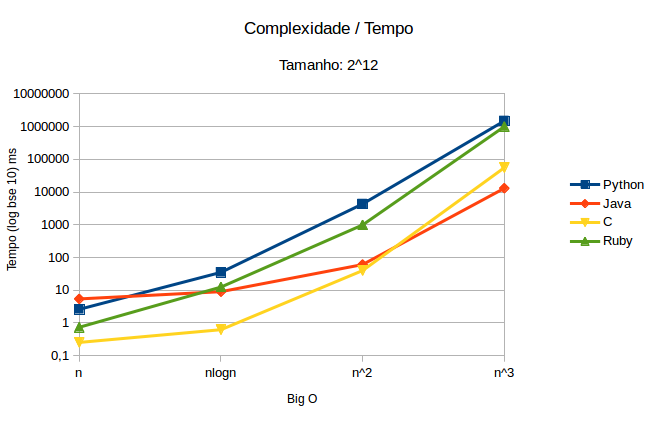
\includegraphics[scale=0.9]{figuras/comp.png} \\
    \caption{Figura 8: Gráfico da complexidade. Programação dinâmica ($n$), Divisão e conquista ($n\log{n}$), Better enumeration ($n^2$) e Enumeration ($n^3$).}
\end{center}




\section{Conclusões}
Conforme a realização das análises de acordo com a complexidade dos algoritmos e seus tamanhos de entrada, os resultados obtidos nos levaram a conclusão de que cada algoritmo se comportou da maneira esperada. É notória a diferença em relação as linguagens de programação, como por exemplo, os tempos de execução dos algoritmos implementados em Python e Ruby, no qual foram semelhantes e consideravelmente mais altos que os algoritmos implementados em C e Java, com exceção do algoritmo implementação de forma dinâmica onde o Java se saiu pior que as demais linguagens. Uma observação interessante é que os testes feitos em Java mostraram uma curva de tempo inferior as outras linguagens. A linguagem C se mostrou na média a mais rápida para todos os casos testados. Por outro lado, Python foi a que demandou mais tempo de execução.
\label{sec:conclusoes}

\newpage


% ----------------------------------------------------------
% ELEMENTOS PÓS-TEXTUAIS
% ----------------------------------------------------------
\postextual
% ----------------------------------------------------------
% Referências bibliográficas
% ----------------------------------------------------------
\renewcommand{\bibsection}{%
\section{\bibname}
\bibmark
%\ifnobibintoc\else
%\phantomsection
%\addcontentsline{toc}{section}{\bibname}
%\fi
\prebibhook}

\bibliography{abntex2-modelo-references}


\newpage
% ----------------------------------------------------------
% Apêndices
% ----------------------------------------------------------

% ---
% Inicia os apêndices
% ---
\begin{apendicesenv}

% ----------------------------------------------------------
\section*{Apêndice A - Execução em Python}
\addcontentsline{toc}{section}{Apêndice A - Execução em Python}
% ----------------------------------------------------------

As tabelas \ref{tab:java1},\ref{tab:java2},\ref{tab:java3} e \ref{tab:java4} apresentam em detalhes os resultados da execução dos
algoritmos Enumeration, Better Enumeration, Divisão e Conquista e Dinâmico em Python:

\begin{table}[!htb]
\centering
\caption{Tempo em milisegundos utilizando o algoritmo Enumeration}
\label{tab:java1}
\footnotesize   %%diminuir tamanho do fonte (-2)
%\small          %%diminuir tamanho de fonte (-1)
\begin{tabular}{l|llllll}
\toprule
& \textbf{$2^7$} & \textbf{$2^8$} & \textbf{$2^9$} & \textbf{$2^{10}$} & \textbf{$2^{11}$} & \textbf{$2^{12}$}\\ 
\midrule
\textbf{Entrada 1} & 42.151 & 310.904 & 2657.217 & 22434.462 & 184035.392 & 1545474.16 \\
\textbf{Entrada 2} & 41.413 & 317.333 & 2672.191 & 22615.633 & 184488.747 & 1476061.11 \\
\textbf{Entrada 3} & 43.539 & 325.1 & 2803.734 & 22721.924 & 184068.904 & 1469058.68\\
\textbf{Entrada 4} & 41.575 & 310.47 & 2698.633 & 22553.105 & 184614.694 & 1479633.35 \\
\textbf{Entrada 5} & 40.886 & 322.595 & 2771.106 & 22960.04 & 185128.694 & 1493786.27 \\
 \bottomrule
\end{tabular}
\end{table}


\begin{table}[!htb]
\centering
\caption{Tempo em milisegundos utilizando o algoritmo Better Enumeration}
\label{tab:java2}
\footnotesize   %%diminuir tamanho do fonte (-2)
%\small          %%diminuir tamanho de fonte (-1)
\begin{tabular}{l|llllll}
\toprule
& \textbf{$2^7$} & \textbf{$2^8$} & \textbf{$2^9$} & \textbf{$2^{10}$} & \textbf{$2^{11}$} & \textbf{$2^{12}$}\\ 
\midrule
\textbf{Entrada 1} & 4.146335 &	16.572707 &	68.384231 &	269.795032 &	1093.729749 &	4416.517415\\
\textbf{Entrada 2} & 4.152714 &	16.686511 &	68.788464 &	272.6177 &	1086.526093 &	4290.938856\\
\textbf{Entrada 3} & 4.163052 &	16.736765 &	68.965081 &	271.764406 &	1084.971064 &	4283.029582\\
\textbf{Entrada 4} & 4.251667 &	18.106293 &	68.465386 &	271.777104 &	1086.896538 & 4305.711889\\
\textbf{Entrada 5} & 4.220251 &	17.631703 &	68.033299 &	271.409339 &	1091.690677 & 4305.382415\\
 \bottomrule
\end{tabular}
\end{table}

\begin{table}[!htb]
\centering
\caption{Tempo em milisegundos utilizando o algoritmo Divisão e Conquista}
\label{tab:java3}
\footnotesize   %%diminuir tamanho do fonte (-2)
%\small          %%diminuir tamanho de fonte (-1)
\begin{tabular}{l|llllll}
\toprule
& \textbf{$2^7$} & \textbf{$2^8$} & \textbf{$2^9$} & \textbf{$2^{10}$} & \textbf{$2^{11}$} & \textbf{$2^{12}$}\\ 
\midrule
\textbf{Entrada 1} & 0.667828 &	1.423543 &	3.046748 &	6.485194 &	14.017516 &	29.307443\\
\textbf{Entrada 2} & 0.798053 &	1.706415 &	3.643792 &	7.883161 &	16.948674 &	35.697267\\
\textbf{Entrada 3} & 0.79769 &	1.678185 &	3.702937 &	7.887057 &	16.965383 &	35.720155\\
\textbf{Entrada 4} & 0.798676 &	1.701212 &	3.668637 &	7.864486 &	17.20358	 & 38.363922\\
\textbf{Entrada 5} & 0.797089 &	1.695006 &	3.815923 &	7.909438 &	16.933554 &	35.674518\\

 \bottomrule
\end{tabular}
\end{table}

\begin{table}[!htb]
\centering
\caption{Tempo em milisegundos utilizando o algoritmo Dinâmico}
\label{tab:java4}
\footnotesize   %%diminuir tamanho do fonte (-2)
%\small          %%diminuir tamanho de fonte (-1)
\begin{tabular}{l|llllll}
\toprule
& \textbf{$2^7$} & \textbf{$2^8$} & \textbf{$2^9$} & \textbf{$2^{10}$} & \textbf{$2^{11}$} & \textbf{$2^{12}$}\\ 
\midrule
\textbf{Entrada 1} & 0.093169 &	0.176887 &	0.329079 & 	0.653361 & 	1.272396 & 	2.70259\\
\textbf{Entrada 2} & 0.093514 &	0.175446 &	0.349052 & 	0.650099 & 	1.27342	 & 2.567602\\
\textbf{Entrada 3} & 0.095778 &	0.179314 &	0.335256 & 	0.685758 & 	1.303668 & 	2.587185\\
\textbf{Entrada 4} & 0.127196 &	0.175583 &	0.34712	 & 1.327424	 & 1.289522	 & 2.559444\\
\textbf{Entrada 5} & 0.094372 &	0.180941 &	0.332899 & 	0.659484 & 	1.295223 & 	2.561774\\
 \bottomrule
\end{tabular}
\end{table}


\end{apendicesenv}
% ---
\newpage
% ---
\begin{apendicesenv}

% ----------------------------------------------------------
\section*{Apêndice B - Execução em C}
\addcontentsline{toc}{section}{Apêndice B - Execução em C}
% ----------------------------------------------------------

As tabelas \ref{tab:java5},\ref{tab:java6},\ref{tab:java7} e \ref{tab:java8} apresentam em detalhes os resultados da execução dos
algoritmos Enumeration, Better Enumeration, Divisão e Conquista e Dinâmico em C:

\begin{table}[!htb]
\centering
\caption{Tempo em milisegundos utilizando o algoritmo Enumeration}
\label{tab:java5}
\footnotesize   %%diminuir tamanho do fonte (-2)
%\small          %%diminuir tamanho de fonte (-1)
\begin{tabular}{l|llllll}
\toprule
& \textbf{$2^7$} & \textbf{$2^8$} & \textbf{$2^9$} & \textbf{$2^{10}$} & \textbf{$2^{11}$} & \textbf{$2^{12}$}\\ 
\midrule
\textbf{Entrada 1} & 4.196 & 21.92 & 24.559 & 941.707 & 7463.329 & 55395.621 \\
\textbf{Entrada 2} & 3.942 & 15.213 & 118.678 &	938.911 & 7463.067 & 55416.682\\ 
\textbf{Entrada 3} & 2.09 & 15.093 & 118.661 &	938.816 & 7502.048 & 55615.719\\ 
\textbf{Entrada 4} & 2.157 & 15.326 & 118.671 &	939.035 & 7493.533 & 55541.399\\ 
\textbf{Entrada 5} & 2.047 & 15.091 & 118.889 &	938.737 & 7476.878 & 55502.526\\ 
 \bottomrule
\end{tabular}
\end{table}


\begin{table}[!htb]
\centering
\caption{Tempo em milisegundos utilizando o algoritmo Better Enumeration}
\label{tab:java6}
\footnotesize   %%diminuir tamanho do fonte (-2)
%\small          %%diminuir tamanho de fonte (-1)
\begin{tabular}{l|llllll}
\toprule
& \textbf{$2^7$} & \textbf{$2^8$} & \textbf{$2^9$} & \textbf{$2^{10}$} & \textbf{$2^{11}$} & \textbf{$2^{12}$}\\ 
\midrule
\textbf{Entrada 1} & 0.043 & 0.162 & 0.633 & 2.492 & 9.932 & 39.699\\
\textbf{Entrada 2} & 0.042 & 0.16 & 0.631 & 2.494 & 9.945 & 39.702\\
\textbf{Entrada 3} & 0.043 & 0.161 & 0.629 & 2.491 & 9.945 & 39.665\\
\textbf{Entrada 4} & 0.042 & 0.161 & 0.629 & 2.495 & 9.956	& 39.82\\
\textbf{Entrada 5} & 0.043 & 0.16 & 0.628 &	2.49 & 9.947 & 39.669\\
 \bottomrule
\end{tabular}
\end{table}

\begin{table}[!htb]
\centering
\caption{Tempo em milisegundos utilizando o algoritmo Divisão e Conquista}
\label{tab:java7}
\footnotesize   %%diminuir tamanho do fonte (-2)
%\small          %%diminuir tamanho de fonte (-1)
\begin{tabular}{l|llllll}
\toprule
& \textbf{$2^7$} & \textbf{$2^8$} & \textbf{$2^9$} & \textbf{$2^{10}$} & \textbf{$2^{11}$} & \textbf{$2^{12}$}\\ 
\midrule
\textbf{Entrada 1} & 0.02 &	0.038 &	0.076 &	0.149 &	0.303 &	0.624\\
\textbf{Entrada 2} & 0.02 &	0.037 &	0.073 &	0.149 &	0.304 &	0.618\\
\textbf{Entrada 3} & 0.019 & 0.037 &	0.073 &	0.152 &	0.308 &	0.639\\
\textbf{Entrada 4} & 0.02 & 0.039 &	0.073 &	0.148 &	0.297 &	0.611\\
\textbf{Entrada 5} & 0.02 & 0.039 &	0.069 &	0.145 &	0.295 &	0.606\\

 \bottomrule
\end{tabular}
\end{table}

\begin{table}[!htb]
\centering
\caption{Tempo em milisegundos utilizando o algoritmo Dinâmico}
\label{tab:java8}
\footnotesize   %%diminuir tamanho do fonte (-2)
%\small          %%diminuir tamanho de fonte (-1)
\begin{tabular}{l|llllll}
\toprule
& \textbf{$2^7$} & \textbf{$2^8$} & \textbf{$2^9$} & \textbf{$2^{10}$} & \textbf{$2^{11}$} & \textbf{$2^{12}$}\\ 
\midrule
\textbf{Entrada 1} & 0.008 &	0.014 &	0.023 &	0.042 &	0.082 &	0.359\\
\textbf{Entrada 2} & 0.007 &	0.012 &	0.023 &	0.04 &	0.099 &	0.367\\
\textbf{Entrada 3} & 0.008 &	0.013 &	0.024 &	0.04 &	0.079 &	0.197\\
\textbf{Entrada 4} & 0.006 &	0.012 &	0.023 &	0.041 &	0.078 &	0.17\\
\textbf{Entrada 5} & 0.006 &	0.012 &	0.024 &	0.041 &	0.08 &	0.171\\
 \bottomrule
\end{tabular}
\end{table}


\end{apendicesenv}
% ---
\newpage
% ---
\begin{apendicesenv}

% ----------------------------------------------------------
\section*{Apêndice C - Execução em Java}
\addcontentsline{toc}{section}{Apêndice C - Execução em Java}
% ----------------------------------------------------------

As tabelas \ref{tab:java9},\ref{tab:java10},\ref{tab:java11} e \ref{tab:java12} apresentam em detalhes os resultados da execução dos
algoritmos Enumeration, Better Enumeration, Divisão e Conquista e Dinâmico em Java:

\begin{table}[!htb]
\centering
\caption{Tempo em milisegundos utilizando o algoritmo Enumeration}
\label{tab:java9}
\footnotesize   %%diminuir tamanho do fonte (-2)
%\small          %%diminuir tamanho de fonte (-1)
\begin{tabular}{l|llllll}
\toprule
& \textbf{$2^7$} & \textbf{$2^8$} & \textbf{$2^9$} & \textbf{$2^{10}$} & \textbf{$2^{11}$} & \textbf{$2^{12}$}\\ 
\midrule
\textbf{Entrada 1} & 9 & 15 & 44 & 220 & 1519 & 11474\\
\textbf{Entrada 2} & 8 & 18 & 49 & 207 & 1551 & 11259\\
\textbf{Entrada 3} & 10 & 19 & 54 & 254 & 1813 & 14209\\
\textbf{Entrada 4} & 8 & 16 & 53 & 199 & 1978 & 14046\\
\textbf{Entrada 5} & 7 & 15 & 45 & 238 & 1793 & 14265\\
 \bottomrule
\end{tabular}
\end{table}


\begin{table}[!htb]
\centering
\caption{Tempo em milisegundos utilizando o algoritmo Better Enumeration}
\label{tab:java10}
\footnotesize   %%diminuir tamanho do fonte (-2)
%\small          %%diminuir tamanho de fonte (-1)
\begin{tabular}{l|llllll}
\toprule
& \textbf{$2^7$} & \textbf{$2^8$} & \textbf{$2^9$} & \textbf{$2^{10}$} & \textbf{$2^{11}$} & \textbf{$2^{12}$}\\ 
\midrule
\textbf{Entrada 1} & 3 & 4 & 8 & 13 & 21 & 63\\
\textbf{Entrada 2} & 3 & 4 & 8 & 15 & 21 & 54\\
\textbf{Entrada 3} & 4 & 6 & 10 & 18 & 25 & 61\\
\textbf{Entrada 4} & 4 & 4 & 11 & 17 & 30 & 62\\
\textbf{Entrada 5} & 3 & 5 & 9 & 19 & 24 & 63\\
 \bottomrule
\end{tabular}
\end{table}

\begin{table}[!htb]
\centering
\caption{Tempo em milisegundos utilizando o algoritmo Divisão e Conquista}
\label{tab:java11}
\footnotesize   %%diminuir tamanho do fonte (-2)
%\small          %%diminuir tamanho de fonte (-1)
\begin{tabular}{l|llllll}
\toprule
& \textbf{$2^7$} & \textbf{$2^8$} & \textbf{$2^9$} & \textbf{$2^{10}$} & \textbf{$2^{11}$} & \textbf{$2^{12}$}\\ 
\midrule
\textbf{Entrada 1} & 3 & 5 & 6 & 8 & 6 & 10\\
\textbf{Entrada 2} & 5 & 5 & 6 & 7 & 9 & 8\\
\textbf{Entrada 3} & 4 & 5 & 6 & 7 & 8 & 10\\
\textbf{Entrada 4} & 3 & 3 & 6 & 8 & 7 & 8\\
\textbf{Entrada 5} & 4 & 3 & 7 & 7 & 8 & 9\\

 \bottomrule
\end{tabular}
\end{table}

\begin{table}[!htb]
\centering
\caption{Tempo em milisegundos utilizando o algoritmo Dinâmico}
\label{tab:java12}
\footnotesize   %%diminuir tamanho do fonte (-2)
%\small          %%diminuir tamanho de fonte (-1)
\begin{tabular}{l|llllll}
\toprule
& \textbf{$2^7$} & \textbf{$2^8$} & \textbf{$2^9$} & \textbf{$2^{10}$} & \textbf{$2^{11}$} & \textbf{$2^{12}$}\\ 
\midrule
\textbf{Entrada 1} & 3 & 3 & 5 & 5 & 5 & 7\\
\textbf{Entrada 2} & 3 & 5 & 4 & 6 & 5 & 5\\
\textbf{Entrada 3} & 5 & 3 & 4 & 6 & 5 & 5\\
\textbf{Entrada 4} & 3 & 3 & 5 & 4 & 6 & 5\\
\textbf{Entrada 5} & 3 & 5 & 5 & 5 & 4 & 5\\
 \bottomrule
\end{tabular}
\end{table}


\end{apendicesenv}

\newpage
\begin{apendicesenv}

% ----------------------------------------------------------
\section*{Apêndice D - Execução em Ruby}
\addcontentsline{toc}{section}{Apêndice D - Execução em Ruby}
% ----------------------------------------------------------

As tabelas \ref{tab:java13},\ref{tab:java14},\ref{tab:java15} e \ref{tab:java16} apresentam em detalhes os resultados da execução dos
algoritmos Enumeration, Better Enumeration, Divisão e Conquista e Dinâmico em Ruby:

\begin{table}[!htb]
\centering
\caption{Tempo em milisegundos utilizando o algoritmo Enumeration}
\label{tab:java13}
\footnotesize   %%diminuir tamanho do fonte (-2)
%\small          %%diminuir tamanho de fonte (-1)
\begin{tabular}{l|llllll}
\toprule
& \textbf{$2^7$} & \textbf{$2^8$} & \textbf{$2^9$} & \textbf{$2^{10}$} & \textbf{$2^{11}$} & \textbf{$2^{12}$}\\ 
\midrule
\textbf{Entrada 1} & 37.475306 &	287.575254 & 2053.913105 & 15859.35741 & 124891.1271 & 1046631.26\\
\textbf{Entrada 2} & 37.578997 &	295.818833 & 2054.799787 & 17472.3414 & 126578.5627 & 993004.1591\\
\textbf{Entrada 3} & 37.018164 &	295.483732 & 2055.586099 & 17264.50218 & 126969.5165 & 994713.8862\\
\textbf{Entrada 4} & 36.973827 & 295.939704 & 2053.536377 & 17264.53854 & 126474.5239 & 991552.6958\\
\textbf{Entrada 5} & 36.993698 & 301.966519 & 2048.703478 & 17261.60135 & 126485.7092 & 991528.896\\

 \bottomrule
\end{tabular}
\end{table}


\begin{table}[!htb]
\centering
\caption{Tempo em milisegundos utilizando o algoritmo Better Enumeration}
\label{tab:java14}
\footnotesize   %%diminuir tamanho do fonte (-2)
%\small          %%diminuir tamanho de fonte (-1)
\begin{tabular}{l|llllll}
\toprule
& \textbf{$2^7$} & \textbf{$2^8$} & \textbf{$2^9$} & \textbf{$2^{10}$} & \textbf{$2^{11}$} & \textbf{$2^{12}$}\\ 
\midrule
\textbf{Entrada 1} & 0.993899 & 4.045848 &	15.901743 &	62.444654 &	257.524619 & 970.600161\\
\textbf{Entrada 2} & 1.019504 & 4.206251 &	15.944256 &	62.815821 &	264.614168 & 994.41845\\
\textbf{Entrada 3} & 1.006231 & 4.019069 &	16.133071 &	62.325197 &	262.938729 & 987.063743\\
\textbf{Entrada 4} & 1.017184 & 4.106712 &	15.370222 &	62.667425 &	262.620891 & 987.714609\\
\textbf{Entrada 5} & 1.020669 & 4.051612 &	15.9196 &	62.395678 &	263.597855 & 988.665379\\
 \bottomrule
\end{tabular}
\end{table}

\begin{table}[!htb]
\centering
\caption{Tempo em milisegundos utilizando o algoritmo Divisão e Conquista}
\label{tab:java15}
\footnotesize   %%diminuir tamanho do fonte (-2)
%\small          %%diminuir tamanho de fonte (-1)
\begin{tabular}{l|llllll}
\toprule
& \textbf{$2^7$} & \textbf{$2^8$} & \textbf{$2^9$} & \textbf{$2^{10}$} & \textbf{$2^{11}$} & \textbf{$2^{12}$}\\ 
\midrule
\textbf{Entrada 1} & 0.323958 &	0.667924 &	1.561697 &	3.269651 &	6.475671 &	13.141231\\
\textbf{Entrada 2} & 0.326489 &	0.692811 &	1.804508 &	2.95368 &	5.794951 &	12.102943\\
\textbf{Entrada 3} & 0.322917 &	0.723338 &	1.480201 &	2.968366 &	6.25653 &	12.076218\\
\textbf{Entrada 4} & 0.3204 &	1.020464 &	1.446125 &	3.151476 &	6.2062 &	12.46555\\
\textbf{Entrada 5} & 0.32245 &	0.718758 &	1.312452 &	3.100121 &	5.931185 &	12.347701\\

 \bottomrule
\end{tabular}
\end{table}

\begin{table}[!htb]
\centering
\caption{Tempo em milisegundos utilizando o algoritmo Dinâmico}
\label{tab:java16}
\footnotesize   %%diminuir tamanho do fonte (-2)
%\small          %%diminuir tamanho de fonte (-1)
\begin{tabular}{l|llllll}
\toprule
& \textbf{$2^7$} & \textbf{$2^8$} & \textbf{$2^9$} & \textbf{$2^{10}$} & \textbf{$2^{11}$} & \textbf{$2^{12}$}\\ 
\midrule
\textbf{Entrada 1} & 0.027963 &	0.050674 &	0.088554 &	0.167804 &	0.330539 &	0.643661\\
\textbf{Entrada 2} & 0.023293 &	0.046227 &	0.090354 &	0.194647 &	0.32373 &	0.688758\\
\textbf{Entrada 3} & 0.022569 &	0.04559 &	0.089591 &	0.1871 &	0.322464 &	0.662466\\
\textbf{Entrada 4} & 0.022253 &	0.045106 &	0.089217 &	0.186277 &	0.321869 &	0.947824\\
\textbf{Entrada 5} & 0.022171 &	0.044891 &	0.088953 &	0.18974 &	0.3219 &	0.729253\\
 \bottomrule
\end{tabular}
\end{table}


\end{apendicesenv}

% ----------------------------------------------------------
% Anexos
% ----------------------------------------------------------

% ---
% Inicia os anexos
% ---
%\begin{anexosenv}

% ---
%\section*{Anexo A - Nome do Anexo}
%\addcontentsline{toc}{section}{Anexo A - Nome do Anexo}
% ---
%\end{anexosenv}


\end{document}
